\chapter{Implementarea Alegria}
\newlength{\bulletwidth}\settowidth{\bulletwidth}{$\bullet$}
\newcommand{\mitem}{\setlength{\leftskip}{\leftmargin}\hspace*{-\labelsep}\hspace*{-\bulletwidth}$\bullet$\hspace*{\labelsep}}
\newcommand{\mend}{\setlength{\leftskip}{0cm}}
\section{Aplicaţia Web}
\begin{wrapfigure}{r}{0.25\textwidth}
	\centering
	\captionsetup{justification=centering}
	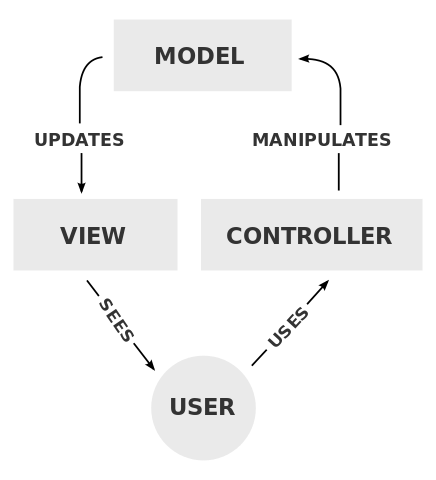
\includegraphics[width=0.25\textwidth]{mvcPattern}
	\caption{Colaborarea intre componentele MVC}
\end{wrapfigure}
Alegria a fost implementata cu ajutorul platformei \textbf{Spring Boot} \autocite{SpringBoot}. Platforma a fost aleasa pentru stabilitatea ei excepţională, fiind bazata pe Spring Framework care sta la baza unora din cele mai mari aplicaţii existente\autocite{springUseCase}, dar si pentru uşurinţa prin care o aplicaţie poate fi compusa din elemente funcţionale, abstractizând peste nivelele de jos a programului, permiţând alocarea timpului pe logica aplicaţiei, si nu pe implementarea platformei pe care aplicaţia sa ruleze.

Cum aplicaţia este bazata pe arhitectura MVC (model-view-controller)  aceasta a fost structurata in trei elemente separate: 

\mitem  \textbf{Interfaţa vizuala}: Realizata in \textbf{HTML5}, folosind motorul de templating Thymeleaf pe server si Bootstrap si JQuery in client pentru afişarea paginilor. Aceasta combinaţie permite realizarea de pagini cu un aspect modern, responsiv, care funcţionează atât pe ecranul mare al calculatorului, cat si pe display-ul mic al unui telefon.

\mitem  \textbf{Modele}: Reprezinta o reprezentare a entităţilor din baza de date in sistemul Alegria.

\mitem  \textbf{Controller-e}: Realizează legătura intre partea vizuala a aplicaţiei si entităţile din baza de date, asigurând atât metodele care "umplu" template-urile cu date, cat si implementarea interfeţei API care introduce si extrage date.

\mend

\subsection{Securitate}
Securitatea este un element de baza, atât pentru accesul la date, cat si pentru accesul la entităţi. Astfel, in implementare s-a folosit framework-ul \textbf{Spring Security} care usureaza management-ul securităţii, fiind puternic integrat si cu restul platformei Spring.
\begin{figure}[H]
	\centering
	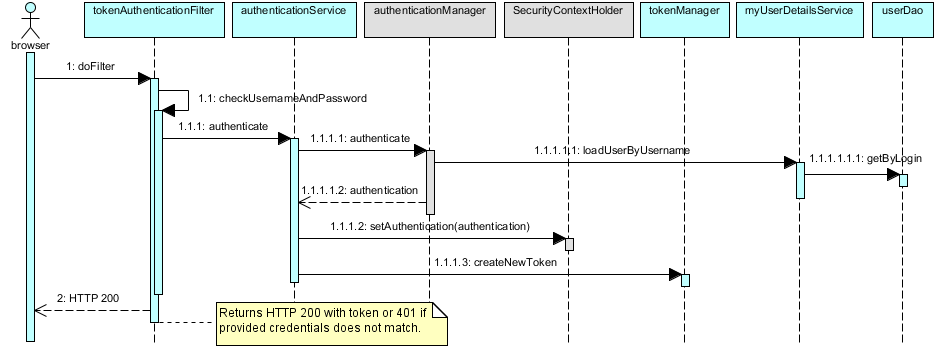
\includegraphics[width=1.35\textwidth, center]{loginUml}
	\caption{Procesul de login in aplicaţie}
	\label{fig:loginUml}
\end{figure}
Pentru autentificare a accesa o resursa protejata, utilizatorul va folosi unul din doua mecanisme:
\begin{itemize}
	\item Autentificare securizata prin username si parola, aceste detalii fiind stocate in tabela \textit{application\_user}, unde parola a fost stocata dupa ce a fost trecuta printr-o funcţie criptografica de hashing. Aceasta metoda de autentificare este folosita pentru autentificarea utilizatorilor in interfaţă de management si monitorizare. Odată ce procesul a reuşit, un token unic va fi generat, iar request-urile următoare vor fi verificate pe baza procesului descris mai jos.
	\item Autentificare pe baza de token, folosita pentru securizarea API-ului, dar si in cazul in care un user s-a autentificat deja cu username si parola. Fiecare request trebuie sa aibă un token, fie într-un cookie, fie ca parametru in url.
\end{itemize}

Tot in scopuri de securitate, fiecare entitate care poate fi modificata menţine un istoric al tuturor modificărilor, împreuna cu utilizatorul cu care le-a efectuat, iar, pentru o dezvoltare ulterioara, accesul unui utilizator poate fi limitat doar la obiectele care au aceleaşi tag-uri ca si utilizatorul.
\subsection{Management}
\begin{figure}[H]
	\centering
	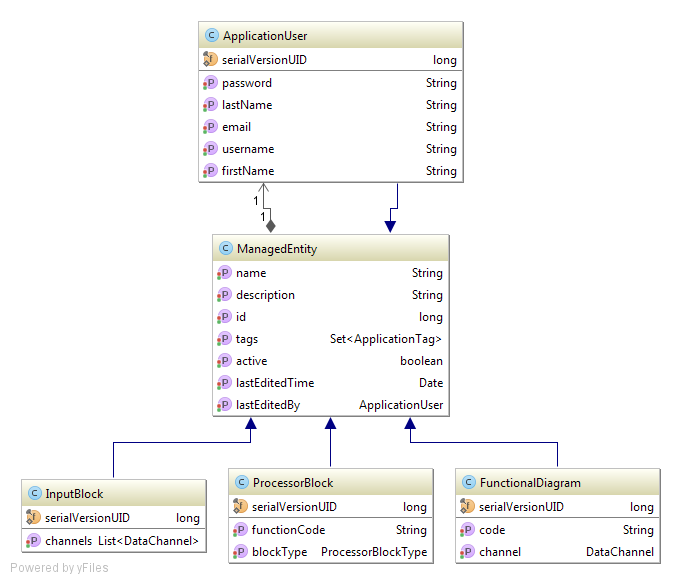
\includegraphics[width=\textwidth, center]{managedEntities}
	\captionsetup{justification=centering}
	\caption{Entităţile care sunt administrate de către utilizator si implementeaza \code{ManagedEntity}}
	\label{fig:managedEntities}
\end{figure}
Toate entităţile care implementeaza \code{ManagedEntity} permit apoi operaţii de adăugare, modificare si ştergere. Acest proces de administrare vizuala foloseşte următoarele resurse, iar un exemplu pentru management-ul :
\begin{itemize}
	\item Un \textbf{repository}, care extinde \code{JpaRepository} din framework-ul Spring Data. Acesta asigura operaţii de căutare, creare, citire, modificare si ştergere a entităţilor. Un avantaj al folosirii  acestui repository, care implementeaza paradigma Data Acces Object (DAO) este ca interacţiunea cu baza de date se face într-un mod consistent si sigur, incompatibilităţile de tip fiind detectate la compilare, si nu la rulare. In Alegria, toate repository-urile folosite, împreuna cu implementările lor se afla in package-ul \code{ro.pub.acse.sapd.repository}.
	\item O \textbf{vizualizare}, template Thyeleaf, care într-o singura pagina HTML expune catre utilizator toate operaţiile suportate de repository. Aceasta pagina este una dinamica, ce foloseşte dialoguri modale încărcate prin AJAX pentru a edita entităţi, fără a fi necesar ca utilizatorul sa fie redirecţionat către o alta pagina. Entităţile sunt afişate sub forma tabelara, dinamica, care permite sortarea si filtrarea după diverse condiţii. Dialogul modal de editare este specific entităţii care este modificate. 
	\item Un \textbf{controller}, clasa cu adnotarea \code{@Controller}, care leagă repository-ul de vizualizare, dar si specifica către Spring care sunt endpoint-urile (căile pe care acest controller le tratează) prin adnotarea \code{@RequestMapping}.
\end{itemize}
\begin{figure}[H]
	\centering
	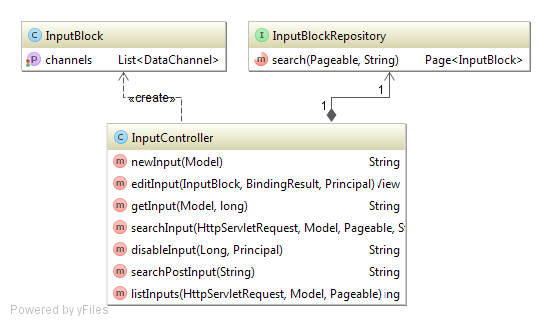
\includegraphics[width=\textwidth, center]{managementInputs}
	\caption{Interacţiunea dintre repository, controller si entitate}
	\label{fig:managementInputs}
\end{figure}

\subsubsection{Managementul blocurilor de intrare}
Pe lângă elementele descrise mai sus, la management-ul blocurilor de intrare trebuie ca utilizatorul sa poată vizualizeze si modifica lista de canale a unui bloc. In vederea implementării acestei particularităţi, in dialogul modal pentru adăugare si modificare a fost realizat un formular dinamic cu cate o line pentru fiecare canal de date. Pentru blocurile de intrare care au deja un canale ataşate, acest formular este generat de către server, in template-ul thymeleaf \code{input.html}, iar, dinamicitatea formularului este implementata cu ajutorul unor funcţii javascript care manipulează structura documentului.


\section{Baza de date}